\chapter{Конструкторский раздел}

%В данном разделе будет проведена формализация сущностей проектируемой системы, описаны используемые домены, ролевая модель и реализуемая табличная функция.

\section{Формализация сущностей системы}
Обозначения в таблицах: PK~---~первичный ключ, FK~---~внешний ключ, U~---~уникальное значение, NN~---~поле не может принимать неопределённое значение, I~---~целочисленный тип, B~---~логический тип, DT~---~тип временной отметки, SP~---~тип временного интервала, S~---~символьный тип, L~---~логический тип, J~---~JSON, ID~---~тип идентификатора.

\paragraph{Таблица Client}\mbox{}

В таблице Client содержится информация о клиентах основной системы. Описание полей таблицы Client представлено в таблице~\ref{table:client}.

\begin{table}[H]
	\begin{center}
		\caption{\label{table:client} Описание полей таблицы Client}
		\begin{tabular}{|l|c|c|c|c|c|l|}
			\hline
			{\specialcell{\\Название}} & \multicolumn{6}{c|}{\specialcell{Характеристики}}\\ \cline{2-7}
			&{PK}&{FK}&{U}&{NN}&{Тип}&{Значение}\\ \hline
			
			id & $+$ & $-$ & $+$ & $+$ & ID & {\specialcell{Идентификатор клиента}}\\ \hline
			name & $-$ & $-$ & $-$ & $+$ & S & {\specialcell{Имя клиента}}\\ \hline
			surname & $-$ & $-$ & $-$ & $+$ & S & {\specialcell{Фамилия клиента}}\\ \hline
			patronymic & $-$ & $-$ & $-$ & $-$ & S & {\specialcell{Отчество клиента}}\\ \hline
			birthDate & $-$ & $-$ & $-$ & $+$ & DT & {\specialcell{Дата рождения}}\\ \hline
			registrationDate & $-$ & $-$ & $-$ & $+$ & DT & {\specialcell{Дата регистрации}}\\ \hline
			gender & $-$ & $-$ & $-$ & $+$ & S & {\specialcell{Пол клиента}}\\ \hline
			email & $-$ & $-$ & $+$ & $+$ & S & {\specialcell{Адрес электронной почты}}\\ \hline
			data & $-$ & $-$ & $-$ & $-$ & J & {\specialcell{Дополнительная информация}}\\ \hline
			
		\end{tabular}
	\end{center}
\end{table}

\newpage

\paragraph{Таблица User}\mbox{}

В таблице User содержится информация о пользователей системы рассылки. Описание полей таблицы User представлено в таблице~\ref{table:user}.

\begin{table}[H]
	\begin{center}
		\caption{\label{table:user} Описание полей таблицы User}
		\begin{tabular}{|l|c|c|c|c|c|l|}
			\hline
			{\specialcell{\\Название}} & \multicolumn{6}{c|}{\specialcell{Характеристики}}\\ \cline{2-7}
			&{PK}&{FK}&{U}&{NN}&{Тип}&{Значение}\\ \hline
			
			id & $+$ & $-$ & $+$ & $+$ & ID & {\specialcell{Идентификатор пользователя}}\\ \hline
			login & $-$ & $-$ & $+$ & $+$ & S & {\specialcell{Логин пользователя}}\\ \hline
			password & $-$ & $-$ & $-$ & $+$ & S & {\specialcell{Пароль пользователя}}\\ \hline
			isAdmin & $-$ & $-$ & $-$ & $+$ & B & {\specialcell{Уровень доступа в системе}}\\ \hline
			
		\end{tabular}
	\end{center}
\end{table}

\paragraph{Таблица Event}\mbox{}

В таблице Event содержится информация о событиях основной системы. Описание полей таблицы Event представлено в таблице~\ref{table:event}.

\begin{table}[H]
	\begin{center}
		\caption{\label{table:event} Описание полей таблицы Event}
		\begin{tabular}{|l|c|c|c|c|c|l|}
			\hline
			{\specialcell{\\Название}} & \multicolumn{6}{c|}{\specialcell{Характеристики}}\\ \cline{2-7}
			&{PK}&{FK}&{U}&{NN}&{Тип}&{Значение}\\ \hline
			
			id & $+$ & $-$ & $+$ & $+$ & ID & {\specialcell{Идентификатор события}}\\ \hline
			alias & $-$ & $-$ & $-$ & $+$ & S & {\specialcell{Идентификатор типа события}}\\ \hline
			clientID & $-$ & $+$ & $-$ & $-$ & ID & {\specialcell{Идентификатор инициатора}}\\ \hline
			eventTime & $-$ & $-$ & $-$ & $+$ & DT & {\specialcell{Время события}}\\ \hline
			
		\end{tabular}
	\end{center}
\end{table}

\paragraph{Таблица EventType}\mbox{}

В таблице EventType содержится информация о типах событий основной системы. Описание полей таблицы EventType представлено в таблице~\ref{table:eventtype}.

\begin{table}[H]
	\begin{center}
		\caption{\label{table:eventtype} Описание полей таблицы EventType}
		\begin{tabular}{|l|c|c|c|c|c|l|}
			\hline
			{\specialcell{\\Название}} & \multicolumn{6}{c|}{\specialcell{Характеристики}}\\ \cline{2-7}
			&{PK}&{FK}&{U}&{NN}&{Тип}&{Значение}\\ \hline
			
			id & $+$ & $-$ & $+$ & $+$ & ID & {\specialcell{Идентификатор события}}\\ \hline
			name & $-$ & $-$ & $-$ & $+$ & S & {\specialcell{Название события}}\\ \hline
			alias & $-$ & $-$ & $+$ & $+$ & S & {\specialcell{Псевдоним события}}\\ \hline
			
		\end{tabular}
	\end{center}
\end{table}

\paragraph{Таблица Ad}\mbox{}

В таблице Ad содержится информация о рекламных записях для рассылки. Описание полей таблицы Ad представлено в таблице~\ref{table:ad}.

\begin{table}[H]
	\begin{center}
		\caption{\label{table:ad} Описание полей таблицы Ad}
		\begin{tabular}{|l|c|c|c|c|c|l|}
			\hline
			{\specialcell{\\Название}} & \multicolumn{6}{c|}{\specialcell{Характеристики}}\\ \cline{2-7}
			&{PK}&{FK}&{U}&{NN}&{Тип}&{Значение}\\ \hline
			
			id & $+$ & $-$ & $+$ & $+$ & ID & {\specialcell{Идентификатор рассылки}}\\ \hline
			content & $-$ & $-$ & $-$ & $+$ & S & {\specialcell{Содержимое записи}}\\ \hline
			filters & $-$ & $-$ & $-$ & $+$ & J & {\specialcell{Фильтры рассылки}}\\ \hline
			createTime & $-$ & $-$ & $-$ & $+$ & DT & {\specialcell{Время создания}}\\ \hline
			userID & $-$ & $+$ & $-$ & $-$ & ID & {\specialcell{Идентификатор создателя}}\\ \hline
			scheduleID & $-$ & $+$ & $+$ & $+$ & ID & {\specialcell{Идентификатор расписания}}\\ \hline
			
		\end{tabular}
	\end{center}
\end{table}

\newpage

\paragraph{Таблица Schedule}\mbox{}

В таблице Schedule содержится информация о расписаниях для рассылок. Описание полей таблицы Schedule представлено в таблице~\ref{table:schedule}.

\begin{table}[H]
	\begin{center}
		\caption{\label{table:schedule} Описание полей таблицы Schedule}
		\begin{tabular}{|l|c|c|c|c|c|l|}
			\hline
			{\specialcell{\\Название}} & \multicolumn{6}{c|}{\specialcell{Характеристики}}\\ \cline{2-7}
			&{PK}&{FK}&{U}&{NN}&{Тип}&{Значение}\\ \hline
			
			id & $+$ & $-$ & $+$ & $+$ & ID & {\specialcell{Идентификатор расписания}}\\ \hline
			nextTime & $-$ & $-$ & $-$ & $+$ & DT & {\specialcell{Время следующей рассылки}}\\ \hline
			span & $-$ & $-$ & $-$ & $+$ & SP & {\specialcell{Интервал рассылки}}\\ \hline
			finished & $-$ & $-$ & $-$ & $+$ & B & {\specialcell{Активность рассылки}}\\ \hline
			periodic & $-$ & $-$ & $-$ & $+$ & B & {\specialcell{Периодичность рассылки}}\\ \hline
			
		\end{tabular}
	\end{center}
\end{table}

\section{Домены}
Для контроля валидности данных введены следующие домены:
\begin{enumerate}
	\item etType~---~временная метка с ограничениями: не позже, чем текущий момент времени.
	\item genderType~---~перечисление, имеющее 2 возможных значения: male, female.
	\item bdType~---~временная метка с ограничениями: не позже, чем текущий момент времени и не ранее, чем 01.01.1900 00:00:00.
	\item rdType~---~временная метка с ограничениями: не позже, чем текущий момент времени, не ранее, чем дата рождения.
	\item loginType~---~символьный тип с ограничениями: не менее 5 символов.
	\item aliasType~---~символьный тип с ограничениями: не менее 5 символов.
	\item ctType~---~временная метка с ограничениями: не позже, чем текущий момент времени.
\end{enumerate}

На рисунке~\ref{img:martin} представлена ER-диаграмма сущностей в нотации Мартина.

\begin{table}[h!]
  \centering
  \begin{tabular}{p{1\linewidth}}
    \centering
    \includegraphics[width=1\linewidth]{./images/martin.pdf}
    \captionof{figure}{ER-диаграмма сущностей в нотации Мартина}
    \label{img:martin}
  \end{tabular}
\end{table}

\section{Ролевая модель на уровне базы данных}
На уровне взаимодействия с базой данных представлена следующая ролевая модель:
\begin{enumerate}
	\item Client~---~пользователь основной системы. Обладает правами на: \begin{itemize}
		\item \texttt{INSERT} в таблицу клиентов Client;
		\item \texttt{INSERT} в таблицу событий Events.
		\end{itemize}
	\item Targetologist~---~таргетолог, координирующий рекламную рассылку. Обладает правами на: \begin{itemize}
		\item \texttt{SELECT}, \texttt{INSERT} в таблицу пользователей User;
		\item \texttt{SELECT}, \texttt{INSERT} в таблицу рассылок Ad;
		\item \texttt{SELECT}, \texttt{INSERT} в таблицу типов событий EventType;
		\item \texttt{SELECT}, \texttt{INSERT}, \texttt{UPDATE} в таблицу расписания Schedule;
		\item \texttt{SELECT} в таблицу клиентов Client;
		\item \texttt{SELECT} в таблицу событий Events.
		\end{itemize}
	\item Administrator~---~администратор системы. Обладает правами на: \begin{itemize}
		\item \texttt{SELECT}, \texttt{INSERT}, \texttt{DELETE}, \texttt{UPDATE} в таблицу пользователей User;
		\item \texttt{SELECT}, \texttt{DELETE} в таблицу клиентов Client.
		\end{itemize}
\end{enumerate}

\section{Разработка табличной функции}
Необходимо разработать табличную функцию, реализующую выборку записей, соответствующих записям о рекламной рассылке, которую необходимо отправить в заданный временной интервал. Записи выбираются из таблицы, сформированной объединением таблицы рассылок Ad с таблицей расписания Schedule.

Схема соответствующей табличной функции \texttt{get\_ads\_by\_span} представлена на рисунке~\ref{img:func}.

\newpage

\begin{table}[h!]
  \centering
  \begin{tabular}{p{1\linewidth}}
    \centering
    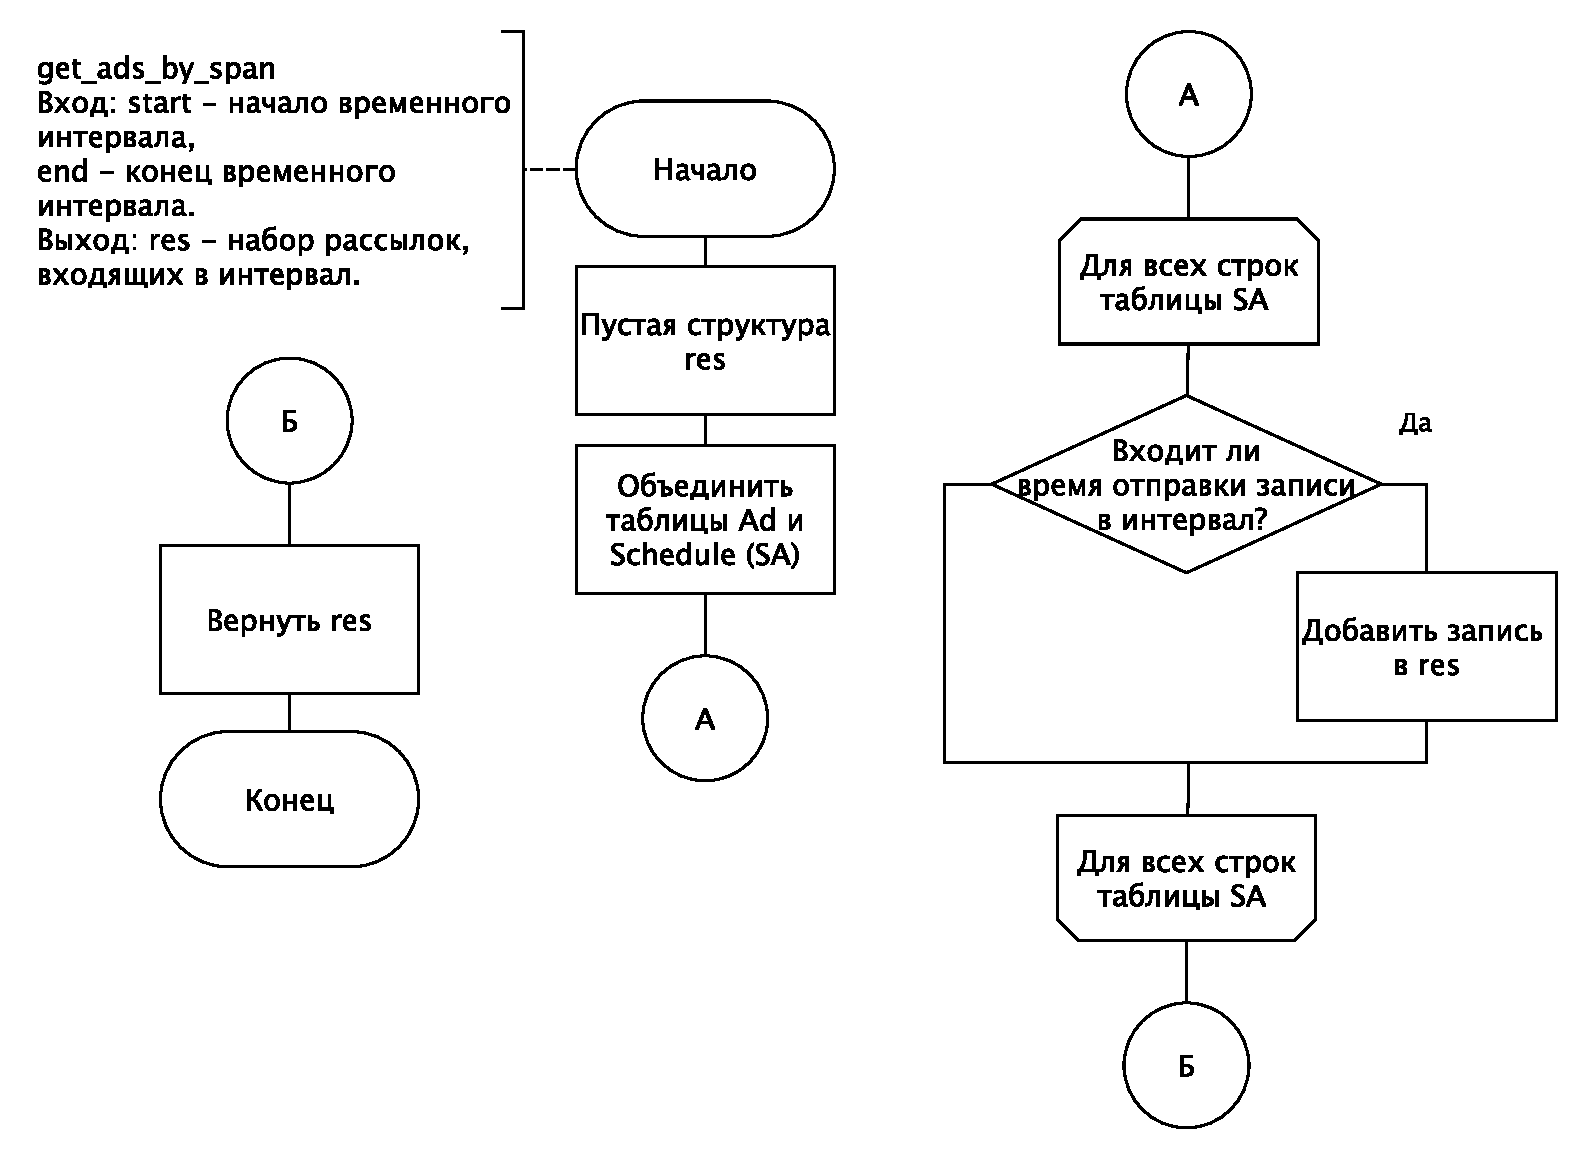
\includegraphics[width=1\linewidth]{./images/func.pdf}
    \captionof{figure}{Схема табличной функции \texttt{get\_ads\_by\_span}}
    \label{img:func}
  \end{tabular}
\end{table}

\section{Вывод}
В данном разделе была проведена формализация сущностей проектируемой системы: на каждую сущность приведена таблица, описывающая её характеристики и необходимые атрибуты. Также, описаны используемые домены, позволяющие поддерживать целостность и непротиворечивость системы, и ролевая модель, определяющая права доступа пользователей к объектам базы данных. Представлена схема алгоритма работы реализуемой табличной функции, осуществляющей выборку записей о рекламной рассылке, которую нужно отправить в заданный интервал времени, реализация которой приведена в листинге Приложения~А.
